\documentclass{mcmthesis}
\usepackage{algorithm}
\usepackage{algorithmic}
\usepackage{physics}
\usepackage{mhchem}
\usepackage{float}
\mcmsetup{
  tcn=2224715,
  problem=A,
  sheet=true,
  titleinsheet=true,
  keywordsinsheet=true,
  titlepage=true,
  abstract=true
}

\makeatletter
\renewcommand{\algorithmicrequire}{\textbf{Input:}}
\renewcommand{\algorithmicensure}{\textbf{Output:}}
\newcommand{\thickhline}{%
    \noalign {\ifnum 0=`}\fi \hrule height 1pt
    \futurelet \reserved@a \@xhline
}
\newcommand{\der}{\mathrm{d}}
\makeatother

\title{Replace with your title}

\begin{document}
  \begin{abstract}
    This is the abstract.
  \end{abstract}

  \begin{keywords}
    keyword1, keyword2
  \end{keywords}
  \maketitle
  \tableofcontents
  \clearpage
  \section{Introduction}
  \subsection{Problem Background}
  Since the first bicycle race was held on the 31 May 1868 at the Parc de Saint-Cloud, Paris, various bicycle games have emerged in large numbers, including road bicycle, tracking cycling, mountain bike and so on. In different kinds of bicycle race, riders are always looking to minimize the time required to cover a given distance.\\
  Besides the fitness of the athletes, appropriate strategies also play a decisive role in a cycling race. A rider can keep a constant speed in the whole game. And he can adjust his speed according to the landform and wind, as well. He can exceed his limits under a certain condition at the price of riding slowly in the next period.\\ 
  However, everyone has different properties in riding. For example, someone may specialize in races that have multiple long climbs (a climber), while another specializes in producing extremely high power for short periods of time (a sprinter). This difference can be described as discrepancy in power curve, which indicates how long a rider can produce a given amount of power. Given a particular rider’s capability according to that rider’s power curve, how should that rider apply power while traversing a given time trial course? \\
  kMoreover, in a team time trial, a team often ride in a line to reduce the air resistance. Given that the team consists of different type of riders, how to arrange the speed of the team and how to arrange the lead rider? These questions are discussed in this paper.\\
  \subsection{Problem Restatement}
  \begin{enumerate}
    \item Develop a model that can be applied to any type of rider that determines the relationship between the rider’s position on the course and the power the rider applies.
    \item Define the power profiles of riders of different types and different genders.
    \item Apply the model on various time trial courses.
    \item Determine the potential impact of weather conditions.
    \item Determine how sensitive the results are to rider deviations from the target power distribution.
    \item Discuss how to extend your model to include the optimal power use for a team time trial.
    \item Write a two-page rider’s race guidance for a Directeur Sportif of a team.
  \end{enumerate}
  
  \subsection{Our Approach}

  \section{Data}
  \subsection{Data Collection}
  The data we used mainly include geographic information of the racing course, typical power curves of different kinds of cyclists.
  The data sources are summarized in Table \ref{tab:data_source}.
  \begin{table}[H]
    \centering
    \caption{Data source collation}
    \label{tab:data_source}
    \begin{tabular}{ccc}
    \thickhline
    Database Names & Database URL & Data Type \\\hline
    Google Earth & \href{https://earth.google.com}{https://earth.google.com} & Geography \\
    SRTM1 & \href{https://www2.jpl.nasa.gov/srtm}{https://www2.jpl.nasa.gov/srtm} & Geography \\
    ODP1 & \href{https://data.opendataportal.at/dataset/dtm-europe}{https://data.opendataportal.at/dataset/dtm-europe} & Geography \\
    \thickhline
    \end{tabular}
  \end{table}

  \subsection{Data Process}

  \subsubsection{Geographic information of the racing course}
  To get the 3D model of the cycling course, we looked up the rider manual. We uniformly sampled points on the racetrack and marked them on Google Earth. In this way, the longitude and latitude information can be exported. Then we reached the elevation information of these points using the database SRTM1 and ODP1.\\
  In order to simplify the data process procedure, we transform the course from terrestrial coordinate system to a space rectangular coordinate system, whose origin locates at the start point and whose $x'$, $y'$, $z'$ axis orient to south, east, sky respectively. The detailed procedures are shown in Fig. \ref{fig:img1}
  \begin{figure}[H]
    \centering
    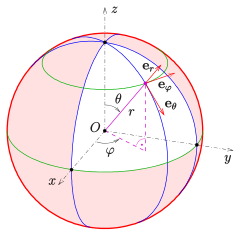
\includegraphics[width=0.4\linewidth]{image/earth_coord}
    \caption{Schematic diagram of the relationship between the ground coordinate system and the right angle coordinate system}%
    \label{fig:img1}
  \end{figure}

  In the old coordinate system shown as $C_{xyz}$ , the coordinate of the start point can be represented as:
  \begin{equation}
    \begin{aligned}
      r_{0} = r_0 \sin \theta_0 \cos \varphi_{0} \hat{x} + r_0 \sin \theta_0 \cos \varphi_0 \hat{y} + r_0 \cos \theta_{0} \hat{z}
    \end{aligned}
  \end{equation}
  where $r_0$ is the coordinate vector of start point in the $C_{xyz}$, $r_0$ is the distance between the start point and he center of the earth $r_0 = R_{e} + h_0$, $R_{e}$ is the radius of the earth, $h_0$ is the elevation of start point; $\theta_0 = \text{latitude-of-startpoint} - 90^\circ$; $\varphi_0$ is he longitude of start point.\\
  The new coordinate is shown in the figure, $C_{e_\theta e_\varphi e_r}$, Its basis vectors can be represented as:
  \begin{equation}
    \left\{
    \begin{aligned}
      &{\bf \hat{e}_{\theta}} = \frac{\sin \theta_0}{|\sin \theta_0|} \cos \theta_0\cos \varphi_0 {\bf \hat{x}} + \frac{\sin \theta_0}{|\sin \theta_0|}\cos \theta_0 \sin\varphi_0 {\bf \hat{y}} - \frac{\sin \theta_0}{|\sin \theta_0|}\sin \theta_0 {\bf \hat{z}} \\
      & {\bf \hat{e}_{\varphi}} = -\sin \varphi_0 {\bf \hat{x}} + \cos \varphi_0 {\bf \hat{y}}\\
      & {\bf \hat{e}_{r}} = \sin \theta_0 \cos \varphi_0 {\bf \hat{x}} + \sin \theta_0 \cos \varphi_0 {\bf \hat{y}} + \cos \theta_{0} {\bf \hat{z}}
    \end{aligned}
    \right.
  \end{equation}
  For the points in he course,
  \begin{equation}
    \begin{aligned}
      {\bf r} &= r\sin \theta \cos \varphi {\bf \hat{x}} + r\sin \theta \cos \varphi {\bf \hat{y}} + r\cos \theta {\bf \hat{z}}\\
              &= ({\bf r}\cdot {\bf \hat{e}_{\theta}}) {\bf \hat{e}_{\theta}} + ({\bf r}\cdot {\bf \hat{e}_{\varphi}}){\bf \hat{e}_{\varphi}} + ({\bf r}\cdot {\bf \hat{e}_{r}}){\bf \hat{e}_{r}}\\
              &= ({\bf r}\cdot {\bf \hat{e}_{\theta}}) {\bf \hat{x}'} + ({\bf r}\cdot {\bf \hat{e}_{\varphi}}) {\bf \hat{y}'} + ({\bf r}\cdot {\bf \hat{e}_{r}}){\bf \hat{z}'}
    \end{aligned}
  \end{equation}

  The coordinate of the points in the new coordinate system is $({\bf r}\cdot {\bf \hat{e}_{\theta}}, {\bf r}\cdot {\bf \hat{e}_{\varphi}}, {\bf r}\cdot {\bf \hat{e}_{r}})$.\\

  As we can see, there are plenty of spines on the figure. The fluctuation of the coordinate is caused of the point sampling on the map. The unrealistic ascent and descent will disturb our simulation to a large extent. To avoid this this problem, we smoothed the data using Gaussian convolution. \\
  For a set of 2-dimensional data $(\xi_{i}, \zeta_{i})$, we can smooth the data with method of weighted average. The weight can be the Gaussian distance between indicator. In this way, the smoothed data can be presented as $(\xi_{j}, \zeta_{j})$ in which
  \begin{equation}
    \begin{aligned}
      \zeta_{j} = \frac{\sum_{i} \zeta_{i} e^{-\frac{(\xi_{i} - \xi_{j})^2}{2 \sigma^{2}}}}{\sum _{i} e^{- \frac{(\xi_{i} - \xi_{j})^{2}}{2 \sigma^{2}}}}
    \end{aligned}
  \end{equation}

  In our data process, we took the trace distance between points and start point as the indicator $\xi_{i}$, and smoothed the $x, y, z$ coordinate respectively. The result is visualized as below. 

  \section{Model}
  \subsection{Model Overview}

  \subsection{Physical Model of Cyclist}
  To simulate the kinetic processes of a cyclist and his/her bicycle, a force analysis is inevitable. In general, the resistance on a cyclist and his/her bicycle includes air drug, air friction, rolling resistance, the downward slope component of gravity. \\
  The air drug is normal to the surface of the resisted body, felling like the pressure of the wind. It can be represented as: 
  \begin{equation}
    \begin{aligned}
      f_{a} = \frac{1}{2} c_{D} \rho S v_{r} ^{2}
    \end{aligned}
  \end{equation}
  The factor $c_D$ is the drag coefficient of air, $\rho$ is the density of air, $S$ is the frontal area of cyclist and his/her bicycle, $v_{r}$ is the relative velocity between air and cyclist. \\
  The air friction is tangential to the surface. For an unstreamlined body such as a bicycle and rider, the pressure effect is much the larger. As a result, the air friction can be ignored.\\
  The rolling resistance can be represented as: 
  \begin{equation}
    \begin{aligned}
      f_{r} = \frac{F_{N} \mu_{R}}{R}
    \end{aligned}
  \end{equation}
  The $F_{N}$ is the pressure of the wheels; $R$ is the radius of the wheels; $\mu_{R}$ is the rolling resistance coefficient, which varies with the condition of the road, the material of the wheel and the air pressure of the pneumatic tire. \\
  The downward slope component of gravity can be represented as: 
  \begin{equation}
    \begin{aligned}
      f_{G} = mg\sin \theta
    \end{aligned}
  \end{equation}
  Where $m$ is the total mass of cyclist and bicycle, $g$ is the gravitational acceleration, $\theta$, is the angle between slope and horizontal. 
  In this way, the kinetic equation of cyclist and bicycle can be represented as:
  \begin{equation}
    \begin{aligned}
      \eta P \dif t = \left[ \frac{1}{2} c_{D} \rho S \left(v - \frac{{\bf v\cdot v_{w}}}{v}\right)^{2} + \frac{mg\cos \theta \mu_{R}}{R} + mg\sin \theta \right]v\dif t + mv \dif v
    \end{aligned}
  \end{equation}
  where $\eta$ is the mechanical efficiency of bicycle, $P$ is the output of the cyclist, ${\bf v,v_{w}}$ is the vector f velocity of cyclist and wind respectively.

  \subsection{Metabolism model of cyclist}
  Cellular respiration is the energy source of human. Aerobic respiration provides most energy we need in quiescent condition and mild exercise. Aerobic respiration resolves organics (glucose mainly), generates water, carbon dioxide and energy. \\
  \begin{equation*}
    \begin{aligned}
      \ce{C6H12O6 ->[{Aerobic respiration}] H2O + CO2 + \text{energy}}
    \end{aligned}
  \end{equation*}
  However, because of the shortage of oxygen, the energy provided by aerobic respiration is not enough when you are doing vigorous exercise. Anaerobic respiration covers the lack in this condition, and its intensity grows with the intensity of exercise. Anaerobic respiration resolves organics (glucose mainly), generates lactic acid and energy.\\
  \begin{equation*}
    \begin{aligned}
      \ce{C6H12O6 ->[{Anaerobic respiration}] C3H6O3 + \text{energy}}
    \end{aligned}
  \end{equation*}
  The energy generation efficiency of anaerobic respiration is much lower than that of aerobic respiration, which means spending same amount of glucose, anaerobic respiration generates less energy than aerobic respiration. Although muscle cells transmit lactic acid to blood constantly, sometimes the generation rate of lactic acid is larger than transition rate, leading to the accumulation of lactic acid. Some scholars believe that is the reason for exhaustion.\\
  In a bicycle game, a cyclist can choose to output a high power at the cost of exhaustion. And he/she can recover by outputting a low power. A cyclist can even exceed his/her limits at certain condition but requires extra time at a lower power level to recover. To describe the exhaustion and recovery of the cyclist in a bicycle game, we designed this metabolism model of cyclist.\\
  Our model gets the cyclist power output history and calculates the cyclist’s physical condition and determines the maximum output power at present.\\
  In our model, the power output is provided by both aerobic respiration and anaerobic respiration. The strength of aerobic respiration has a maximum which changes with the lactic acid concentration (considering the metabolic waste effects the blood’s ability of carrying oxygen). If the needed output power is smaller than this maximum, then 95\% power is provided by aerobic respiration and the rest provided by anaerobic. If the needed output power is larger than this maximum, then aerobic respiration provides its maximum power and the rest is provided by anaerobic respiration. The anaerobic respiration also has a maximum which changes largely. We take the concentration of lactic acid in muscle cell as constraint of muscle cell’s anaerobic respiration. The maximum power generated by anaerobic respiration decreases linearly with the increase of lactic acid concentration in muscle cell. And if the lactic acid concentration exceeds a typical threshold, the energy generation efficiency of anaerobic respiration is halved, which means muscle cell needs double glucose and generates double lactic acid for the same energy.\\


  \subsection{Optimize Model}
  Our optimization model combines the metabolic model of the cyclist with the physical model, to optimize the cyclists' power distribution over the entire course of the track respect to the time taken by the cyclist to complete the track as target function.\\ We use Differential Evolution algorithm to optimize this problem, as shown below
  \begin{algorithm}
    \caption{Differential Evolution algorithm to optimize the power distribution}
    \label{alg:DE}
    \begin{algorithmic}
      \REQUIRE ~~\\
      The population of random generated power distribution, $N_P$;\\
      The zoom factor,  $F$;\\
      The crossover probability $cr$;
      The possible power specify by doundary $lb$ and $hb$ ;\\
      The track parameters and cyclist parameters, $T_p$, $C_p$;
      \ENSURE ~~\\
      Optimal power distribution, $P(x)$;\\
      $X_{i,j}$ = $lb$ + random() $\times$ ($hb$-$lb$), $i\in 1,\cdots,N_P$;\\
      \WHILE {the termination condition is not statisfied}
      \FOR{$j \in (1,N_P)$}
      \STATE Randomly generate 3 integers $r_1, r_2, r_3\in (1,N_P)$
      \FOR {each paramters $i$}
      \IF {rand(0,1) < CR or $i=i_{rand}$}
      \STATE $x_{i,j} = x_{i,r_1} + F\times (x_{i,r_2} - x_{i,r_3})$
      \ELSE
      \STATE $x_{i,j} = x_{i,j}$
      \ENDIF
      \ENDFOR
      \ENDFOR
      \ENDWHILE
    \end{algorithmic}
  \end{algorithm}
  The following figure visualizes how the Differential Evolution algorithm takes random points in the phase space, calculates the mutation vector, and exchanges the components with the current state with a certain probability


  \section{Stability Analyze}
  \subsection{Wind influence}
  In order to study the effect of wind speed and wind direction on cyclists' race performance, we first need to obtain the optimal power distribution of cyclists in the absence of wind. After that, we calculate the time required to complete the race with this power distribution for different wind speeds and directions. We uniformly take the east-west and north-south winds from -10m/s to 10m/s, and their combinations, and then calculate the variation of the cyclist's time needed to finish the race under each weather condition, and plot it in the heat map below.
  
  \end{document}
